\section{Regular Type Expressions}

\begin{frame}{Regular Type Expressions}
  \centering
  
  
\includegraphics[width=0.9\textwidth]{regexp.png}
\end{frame}


\newsavebox\exnotebox
\begin{lrbox}{\exnotebox}
  \begin{minipage}{7cm}
    %% dont re-indent this file
\begin{lstlisting}[style=scalaioScala]
val I:Rte = Atomic(classOf[Int])
val F:Rte = Atomic(classOf[Float])
val D:Rte = Atomic(classOf[Double])

val re:Rte = (I ++ (D | F).+).*
\end{lstlisting}

  \end{minipage}
\end{lrbox}


\begin{frame}{RTEs}{What are Regular Type Expressions?}
  \begin{itemize}
  \item A Regular Type Expression (RTE) is an \emph{expression} designating a set  of finite sequences.
  \item Mathematical notation
    \[Int^* \cdot (String \vee Boolean)^*\]
  \item Scala notation\\
    \usebox\exnotebox
  \end{itemize}
\end{frame}

\begin{frame}{levels}{Three levels of RTE}
  The set of all RTEs is recursively defined.
  \begin{itemize}
  \item leaf level
  \item recursive
  \item extended
  \end{itemize}
\end{frame}

\newsavebox\leafbox
\begin{lrbox}{\leafbox}
  \begin{minipage}{12cm}
    %% dont re-indent this file
\begin{lstlisting}[style=scalaioScala]
EmpySet   // empty set of sequences.
Sigma     // singleton sequences.
EmptyWord // empty sequences.

// singleton sequences of Int and of String
val Int:Rte = Atomic(classOf[Int])    
val Str:Rte = Atomic(classOf[String])

Int.contains(List(42))      // returns true
Int.contains(List("hello")) // returns false
Str.contains(List("hello")) // returns true
Str.contains(List())        // returns true
\end{lstlisting}

  \end{minipage}
\end{lrbox}

\begin{frame}{Leaf}
  \usebox\leafbox
\end{frame}

\newsavebox\orbox
\begin{lrbox}{\orbox}
  \begin{minipage}{12cm}
    %% dont re-indent this file
\begin{lstlisting}[style=scalaioScala]
val r1:Rte = Or(EmptySeq, Int, Str)
val re:Rte = EmptySeq | Int | Str
      
re.contains(List(42)) // returns true
re.contains(List("hello")) // returns true
re.contains(List(42, "hello")) // returns false
\end{lstlisting}

  \end{minipage}
\end{lrbox}

\newsavebox\catbox
\begin{lrbox}{\catbox}
  \begin{minipage}{12cm}
    \begin{lstlisting}[style=scalaioScala]
val r1:Rte = EmptyWord | Int | str
val r2:Rte = Cat(Int, Str, r1)
val r2:Rte = Int ++ str ++ r1

r2.contains(List(42, "hello")) // returns true
r2.contains(List(42, "hello", 42)) // returns true
r2.contains(List("hello", 42)) // returns false
\end{lstlisting}

  \end{minipage}
\end{lrbox}


\begin{frame}{Recursive}{Union, Or}
  \usebox\orbox
 \end{frame}

\begin{frame}{Recursive}{Concatenation}
  \usebox\catbox
 \end{frame}



\newsavebox\starbox
\begin{lrbox}{\starbox}
  \begin{minipage}{12cm}
    %% dont re-indent this file
\begin{lstlisting}[style=scalaioScala]
val r3:Rte = Star(Int) // or Int.*
r3.contains(List(1,2,3,4,5)) // returns true

val r4:Rte = Star(Str) // or Str.*
r4.contains(List("a", "b", "c")) // returns true
r4.contains(List(1, "hello", 2, 3, "world") // return false

val r5:Rte = Star(Int | Str) 
r5.contains(List(1, "hello", 2, 3, "world") // return true
\end{lstlisting}

  \end{minipage}
\end{lrbox}


\begin{frame}{Recursive}{Repetition, Star}
  \usebox\starbox
\end{frame}


\newsavebox\extendedbox
\begin{lrbox}{\extendedbox}
  \begin{minipage}{12cm}
  %% dont re-indent this file
\begin{lstlisting}[style=scalaioScala]
// binary infix operators
r1 & r2 == And(r1,r2)
r1 | r2 == Or(r1,r2)
r1 ++ r2 == Cat(r1,r2)

// complement (unary)
!re == Not(re)

// one/zero or more, optional
re.* == Star(re)
re.+ == re ++ re.*
re.? == EmptySeq | re

// exponent, n-times
re^4 == re ++ re ++ re ++ re
\end{lstlisting}

  \end{minipage}
\end{lrbox}

\begin{frame}{Extended RTEs}{Mostly Syntax Sugar}
  \usebox\extendedbox
\end{frame}


\newsavebox\exampleAbox
\begin{lrbox}{\exampleAbox}
  \begin{minipage}{12cm}
    %% dont re-indent this file
\begin{lstlisting}[style=scalaioScala]
val data = Seq("C", 100, 200, 300,
               "M", 10.0, 20.0,
               "M",
               "C", 1, 2, 3,
               "C", -1, -3, -7, -8)
\end{lstlisting}

  \end{minipage}
\end{lrbox}

\newsavebox\exampleAbbox
\begin{lrbox}{\exampleAbbox}
  \begin{minipage}{12cm}
    %% dont re-indent this file
\begin{lstlisting}[style=scalaioScala]
val data = Seq("C", 100, 200, 300, // count
                 "M", 10.0, 20.0, // measurement
                 "M",
                 "C", 1, 2, 3,
                 "C", 1, 3, 7, 8)

val F:Rte = Atomic(classOf[Double]) | Atomic(classOf[Float])
val I:Rte = Atomic(classOf[Int])
val keyM:Rte = Eql("M")
val keyC:Rte = Eql("C")

val re:Rte = ((keyC ++ I.*) | (keyM ++ F.*)).*

re.contains(data) // returns true
\end{lstlisting}

  \end{minipage}
\end{lrbox}

\newsavebox\exampleAcbox
\begin{lrbox}{\exampleAcbox}
  \begin{minipage}{12cm}
    %% dont re-indent this file
\begin{lstlisting}[style=scalaioScala]
val bad   = Seq("C", 100, 200, 300,
                 "M", 10.0, 20.0,
                 "M",
                 "C", 1, ~~2.0~~, 3, // VIOLATES PATTERN
                 "C", 1, 3, 7, 8)

val F:Rte = Atomic(classOf[Double]) | Atomic(classOf[Float])
val I:Rte = Atomic(classOf[Int])
val keyM:Rte = Eql("M")
val keyC:Rte = Eql("C")

val re:Rte = ((keyC ++ I.*) | (keyM ++ F.*)).*

re.contains(~~bad~~) // returns false
\end{lstlisting}

  \end{minipage}
\end{lrbox}

\newsavebox\exampleAdbox
\begin{lrbox}{\exampleAdbox}
  \begin{minipage}{12cm}
    %% dont re-indent this file
\begin{lstlisting}[style=scalaioScala]
val F:Rte = Atomic(classOf[Double]) | Atomic(classOf[Float])
val I:Rte = Atomic(classOf[Int])
val keyM:Rte = Eql("C")
val keyC:Rte = Eql("M")

val re:Rte = ((keyC ++ I.*) | (keyM ++ F.*)).*
\end{lstlisting}

  \end{minipage}
\end{lrbox}


\begin{frame}{Example}{An RTE to match}
  \usebox\exampleAbox

  \begin{itemize}
  \item Keyword strings \code{"C"} and \code{"M"}
  \item \code{"C"} followed by zero or more \code{Int} values
  \item \code{"M"} followed by zero or more values, \code{Double} or \code{Float}
  \end{itemize}
\end{frame}

\begin{frame}{Example}{Successful match}
  \usebox\exampleAbbox
\end{frame}

\begin{frame}{Example}{Does not match}
  \usebox\exampleAcbox
\end{frame}

\begin{frame}{Example}{DFA}
  \usebox\exampleAdbox
  
  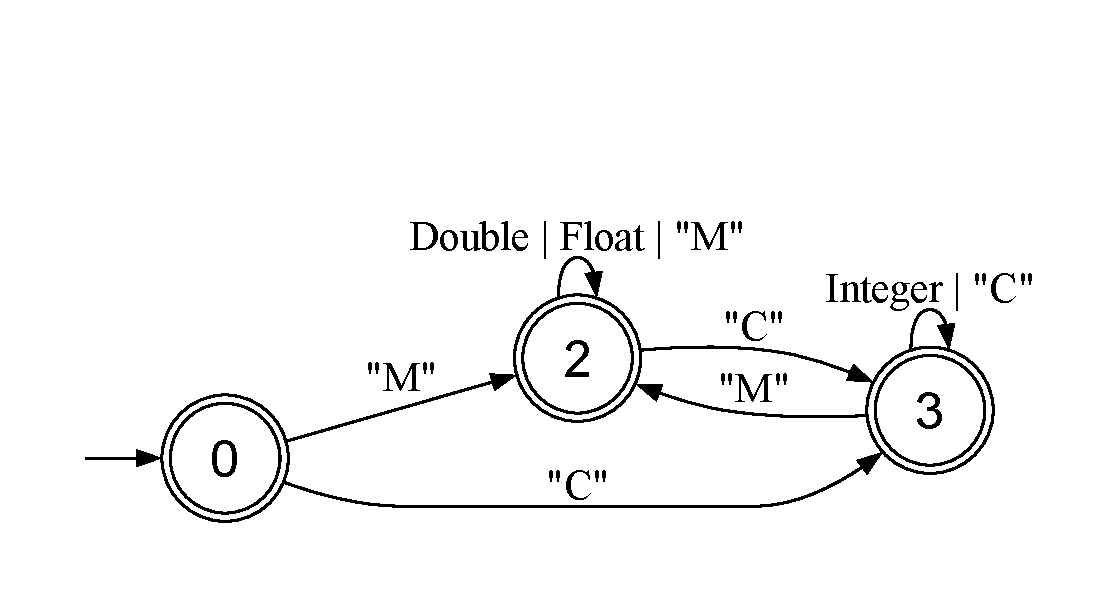
\includegraphics[width=0.9\textwidth]{example2.pdf}
\end{frame}

